\section{Characterization Problem Results}
\label{sec:CharResults}

To quantify the $\Omega$-method success for a variety of anisotropy-inducing
physics, we will present various forms of the Figure of Merit, as described in
Section \ref{sec:successmetrics}.
In the preceding subsections, a
subset of flux anisotropy-inducing physics have been identified
and a subset of problems that contain these physics have been conceptualized.
In this section, the results for CADIS-$\Omega$, CADIS, and nonbiased Monte Carlo
will be presented for each of these problems. Note that the default
deterministic parameters for each problem are used and each Monte Carlo run is
defaults to use the same particle count. Times to transport this particle
quantity between methods due to differences in sampling. Monte Carlo and ADVANTG
inputs are provided in Appendix \ref{sec:github_codes}.

\begin{table}[h!]
  \centering
  \begin{tabular}{l|m{5cm}}
\toprule
Parameter Type & Parameter Value \\
\midrule \midrule
\multicolumn{2}{c}{ADVANTG Values$^1$} \\
\midrule
P$_N$ Order               &    $3$ \\
Quadrature Type           &  Quadruple Range \\
Quadrature Order          &    $10$ \\
Spatial Solver            &  Step Characteristic \\
Energy Group Library$^{\dagger}$     &    27G19N \\
Boundary Conditions & vacuum \\
\midrule \midrule
\multicolumn{2}{c}{MCNP Values$^2$} \\
\midrule
Particle Count      &   $1e7$ \\
Boundary Conditions & vacuum \\
\bottomrule
\end{tabular}
\begin{flushleft}
\footnotesize{
  $^1$ ADVANTG runs of the characterization problems
  were run on 16 cores of a 32 core node, with 256Gb of memory on
  an Oak Ridge National Laboratory compute cluster maintained by the Radiation
  Transport and Nuclear Systems Division. \\
  $^2$ MCNP runs of the characterization problems were run on the same
 machine, with 256Gb of memory but using all 32 cores of the node. \\
  $^{\dagger}$ Parameter type that has no default in ADVANTG.}
\end{flushleft}


  \caption[Default simulation values for characterization problems.]{
    Default simulation values for the characterization problems. The values for
    ADVANTG primarily signify parameters used to run Denovo, with exceptions for
    calculating biasing parameters, which is done exclusively in ADVANTG.
    MCNP-specific values are those used for Monte Carlo runs.
  }
  \label{tab:simulation_defaults}
\end{table}
[Describe default deterministic and monte carlo specs for problems.]

\subsection{Maze Variants}
\label{subsec:resultsmaze}
\subsubsection{Single Turn}
[Table of FOMs for this problem] \\

\begin{table}[h!]
  \centering
  \begin{tabular}{lrrrrr}
\toprule
{} & cadis &             & cadisangle &             & analog \\
{} &    MC & MC\_adjusted &         MC & MC\_adjusted &     MC \\
\midrule
tally avg   &   327 &         248 &        224 &          71 &  0.054 \\
max RE      &  1.46 &        1.11 &       1.02 &       0.322 & 0.0393 \\
min RE      &   113 &        85.6 &         71 &        22.5 &    -- \\
time (mins) &  51.5 &          68 &       35.5 &         112 &   25.5 \\
\bottomrule
\end{tabular}

  \caption[Figure of Merit comparison for single turn maze.]{The FOMS are
  quantified using three relative error results and two different timing results.
  The relative errors used are the tally average relative error, the tally maximum relative
  error, and the tally minimum relative error; the times are total walltimes for
  the Monte Carlo calculation and the sum of the hybrid method software, the
  deterministic tranport time, and the Monte Carlo calculation time.}
  \label{tab:maze1foms}
\end{table}

[Plot of tally results for this problem] \\

\begin{figure}[h!]
  \centering
  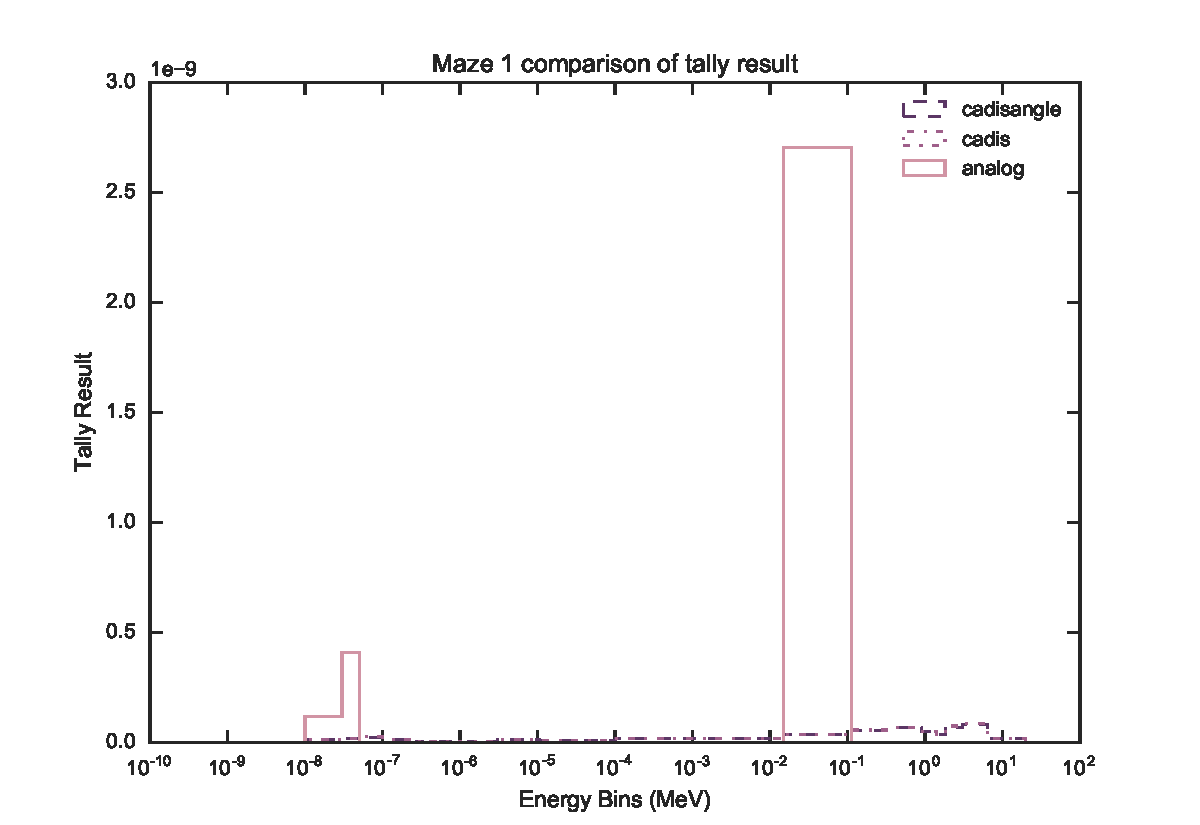
\includegraphics[height=10cm]{./chapters/characterization_probs/figures/maze1/maze_1_tally_result_compare.pdf}
  \caption[Tally results comparison between methods for single turn labyrinth.]
  {This is a fun tally result.}
  \label{fig:maze1result}
\end{figure}

\begin{figure}[h!]
  \centering
  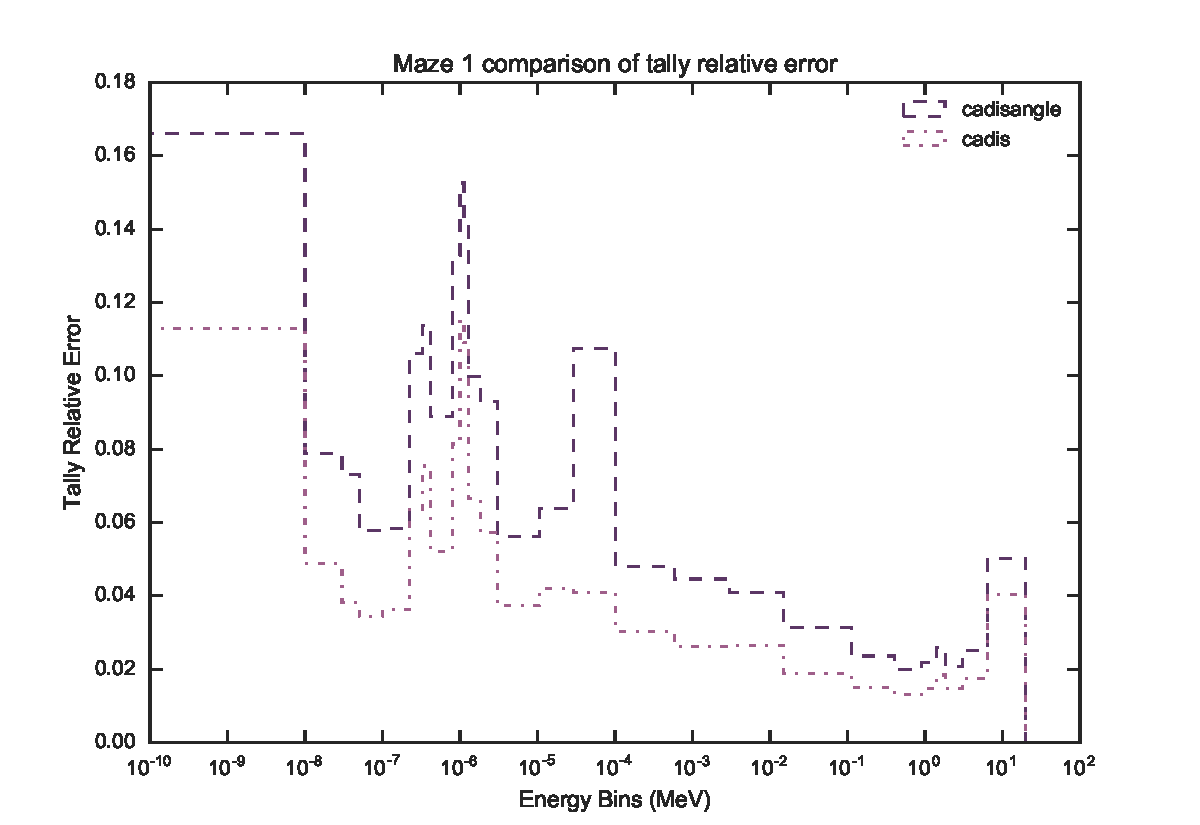
\includegraphics{./chapters/characterization_probs/figures/maze1/maze_1_tally_error_compare.pdf}
  \caption[Tally relative error comparison between methods for single turn
  labyrinth]{This is a super cool result.}
  \label{fig:maze1result}
\end{figure}
[Plot of anisotropies for this problem] \\

[Summarize results and describe issues affecting performance] \\

\subsubsection{Multiple Turn}
[Table of FOMs for this problem]\\

[Plot of tally results for this problem]\\

[Plot of anisotropies for this problem] \\

[Summarize results and describe issues affecting performance] \\

\subsection{Steel Beam}
\label{subsec:resultbeam}
[Table of FOMs for this problem] \\

[Plot of tally results for this problem] \\

[Plot of anisotropies for this problem] \\

[Summarize results and describe issues affecting performance] \\

\subsection{U-Shaped Corridor}
\label{subsec:resultsucorridor}
[Table of FOMs for this problem] \\

[Plot of tally results for this problem] \\

[Plot of anisotropies for this problem] \\

[Summarize results and describe issues affecting performance] \\

\subsection{Shielding with Rebar}
\label{subsec:resultrebar}
[Table of FOMs for this problem] \\

[Plot of tally results for this problem] \\

[Plot of anisotropies for this problem] \\

[Summarize results and describe issues affecting performance] \\

\subsection{Beam Problem}
\label{subsec:resultsbeam}
[Table of FOMs for this problem] \\

[Plot of tally results for this problem] \\

[Plot of anisotropies for this problem] \\

[Summarize results and describe issues affecting performance] \\

\subsection{Therapy Room}
\label{subsec:resultstherapy}
[Table of FOMs for this problem] \\

[Plot of tally results for this problem] \\

[Plot of anisotropies for this problem] \\

[Summarize results and describe issues affecting performance] \\

